\documentclass[12pt]{article}
\usepackage{amsmath}
\usepackage{amssymb}
\usepackage{graphicx}
\usepackage{comment}
\usepackage{longtable}
\usepackage{graphicx}

\begin{document}

\title{\textbf{SOFTWARE ARCHITECTURE DOCUMENT }}
\maketitle

\begin{center}
\title{\textbf{Software Design COMS3009}}
\maketitle
\end{center}
\begin{center}
\title{\textbf{FindMeTutor Android Application}}
\maketitle
\end{center}

\begin{center}
Proposed idea by:\\
Shaneel James-718840
\\Jadon Manilal-815050
\\Jared Naidoo - 719238
\\Krupa Prag - 782681
\\Nivek Ranjith - 802119
\end{center}


\newpage
%TABLE OF CONTENTS
\tableofcontents
\newpage


\section{\textbf{Introduction}}
%\begin{flushleft}
\begin{itemize}

\item Purpose\\
The Software Architecture Document (SAD) provides a comprehensive architectural overview of the FindMeTutor system. It presents a number of different architectural views to depict different aspects of the system. It is intended to capture and depict the different architectural decisions that have been made.

\item Scope\\
The scope of the SAD is to depict the architecture of the FindMeTutor system. This includes the FindMeTutor tutor application, FindMeTutor student application and the backend system that allows FindMeTutor to operate.

\item Definitions, Acronyms and Abbreviations\\
UML: Unified Modeling Language\\
SAD: Software Architecture Document

\item Overview\\
This document provides the reader with a deeper understanding of the FindMeTutor system. It is organised into several views of the system. These views include the Logical View, Deployment View, Implementation view and the Data View.


\end{itemize}

%\end{flushleft}
\pagebreak

\section{Architecture}
This section contains a description pertaining to the architecture used in the FindMeTutor system.

\begin{itemize}
\item Type of Architecture\\
The FindMeTutor system makes use of 2-Tier architecture. The application layer contains the user-interface and the business logic. The second layer contains the database ,which stores the user data for the system. Below is a diagram which depicts the selected architecture:\\
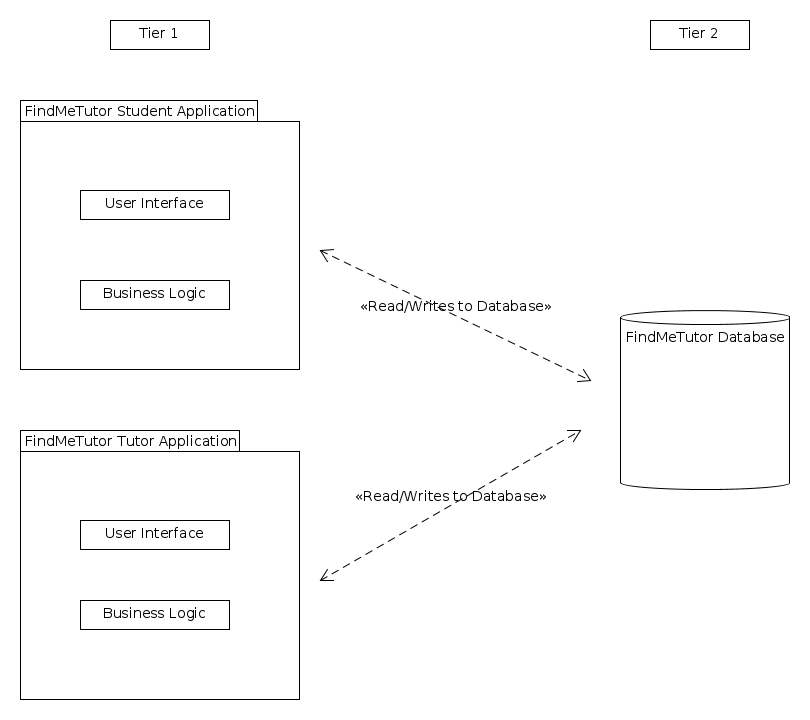
\includegraphics[width=140mm]{./2_Tier_Diagram.png}\\

\item Advantages of 2-Tier Architecture
\begin{itemize}
\item Allows the application to be easily devloped due to the architectures simplicity.
\item Maximum user satisfaction can be ensured due to accurate and fast prototyping of applications.
\item Database logic and business logic are physically close, which offers higher performance.\\
\end{itemize}

\item Responsibilities of Layer 1 (Application Level):
\begin{itemize}
\item The application layer contains the businnes logic and user interface. The first layer is responsible for conveying FindMeTutor services to the client. Layer 1 contains the administration layer used to add funds to a student/tutor account as well as general configuration by an approved administrator.
\end{itemize}

\item Responsibilities of Layer 2:
\begin{itemize}
\item Contains the data for the system. Allows multiple users to access the same data simultaneously.
\end{itemize}

\item Systems of interest\\
The main systems of interest is FindMeTutor which contain the following two subsystems:
\begin{itemize}
\item FindMeTutor Student Application
\item FindMeTutor Tutor Application
\end{itemize}

\item Supplementary Information\\
The FindMeTutor system comprises of two main components: The FindMeTutor student application and the FindMeTutor tutor application. The student application is used by the students to manage anything related to a student account and the tutor application is used by the tutors to manage anything related to the tutor account.Requests for a tutor are made using the student application and responses from tutors as to whether to accept or reject the requests are made using the tutor application.
\end{itemize}

\pagebreak

\section{Architectural Goals and Constraints}
The following lists the goals and constraints of the FindMeTutor system.
\begin{itemize}

\item Technical Platform\\
The FindMeTutor application will be deployed on the Android mobile platform. The application is made up of two parts the user interface and the businness logic. The application then communicates with a server of which the entire systems data is stored. The database system consists of an Ubuntu server running a MySql databse.

\item Transcations
\begin{itemize}

\item Student Transcation\\
The student would pay funds into the FindMeTutor bank account. The students email address would be used as a reference. As soon as the funds have cleared the student is provided with a credit on the FindMeTutor system. The student can then use the credit to book and pay for tutoring sessions.

\item Tutor Transaction\\
Upon a successful tutoring session. The FindMeTutor system credits the tutor with the amount agreed upon. All of the tutors credits are added up at the end of the month and then paid out to the tutor by means of a bank transfer.
\end{itemize}

\item Security\\
The FindMeTutor system takes security very seriously. During a tutoring session the systems logs the exact GPS location of both the tutor and student at all times. Should a location not be logged by both the student and tutor. The the tutor will not receive payment and the student will receive a poor rating.Further communication with FindMeTutor will be required by the tutor to receive payment.

\item Reliability/Availability (failover)\\
The FindMeTutor system makes use of a failover or backup server in the event that something should go wrong. Furthermore FindMeTutor has made aquired additional capacity so as to anticipate an uptake in system usage and as a result ensure the system is reliable at all times.
\end{itemize}

\pagebreak

\section{Stakeholders}
This section lists the various organisations who are concerned with the project.
\begin{itemize}

\item Development Team (Stakeholder 1)\\
The Development team is concerned with the implementation of the system, they want to develop the designed system in the best possible way.

\item Analysts (Stakeholder 2)\\
The analysts are concerned with the design of the system, and the functionality of the system.

\item Lecturer (Stakeholder 3)\\
The Software Design lecturer is concerned with the progress of the designing and implementation of the system.

\item Students (Stakeholder 4)\\
Students want a system which will address their needs as well as a proper functioning system which is favourable towards them finding tutors.

\item Tutors (Stakeholder 5)\\
Tutors want a system which addresses their needs as well as a proper functioning system which is favourable towards them as they wish to earn an income from FindMeTutor.
\end{itemize}

\pagebreak

\section{Concern and Stakeholder Traceability}
\subsection{Concerns}
This section identifies concers relating to the architecture of the FindMeTutor system.
\begin{itemize}

\item Purpose of the system (Concern 1)\\
The main purpose of the system is to provide a connection between a student and a tutor.A potential concern here would be a slow uptake or worse students are not interested in using the application.

\item Suitability of the architecture (Concern 2).\\
The two tier architecture selected allows the developers to modify different aspects of the system without affecting other important aspects of the system. For example: if the businness logic should change, we can simply modify the logic layer of the application while not affecting the user interface or database layers of the application/system.\\\\A potential concern here would be that the architecture above does not fully support certain aspects of expansion should the system experience growth and need to be expanded

\item Feasibility (Concern 3)\\
Should the system not be feasible. i.e. High costs of keeping the system running. Developers and server costs for the system would be high and FindMeTutor would need some sort of revenue to keep the system running. Scability is another issue, we need to scale in order to create revenue. A concern would be that the system does not create revenue for the upkeep of the system and hence the system is no longer feasible.

\item Evolution of the FindMeTutor system (Concern 4)\\
The system will change as time progress, the system is largely based on the users of the system. Thus as the users change, the system will have to change to match the users. A concern here would be that system does not meet the users demands/preferences and ultimately fails.
\end{itemize}

\subsection{Traceability Matrix}
The following table depicts the relationship between the concerns listed above and the various stakeholders of the FindMeTutor system listed in the previous section.\\\\
Stakeholder 1 - Development Team\\
Stakeholder 2 - Analysts\\
Stakeholder 3 - Lecturer\\
Stakeholder 4 - Students\\
Stakeholder 5 - Tutors\\\\
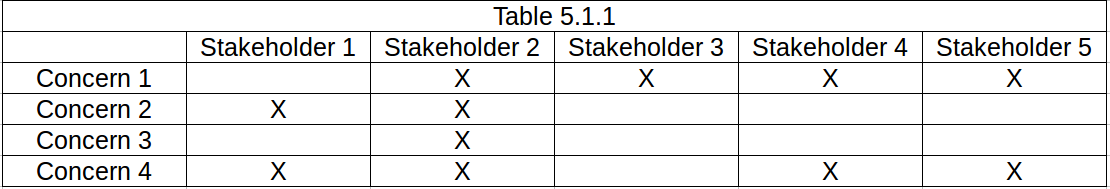
\includegraphics[width=140mm]{./trace.png}

\section{Views}
Description of the different views:
%Listed below are views which.
\begin{itemize}
\item Logical View
The logical view is concerned with the functionality that the system provides to end users. The view includes diagrams such as the class diagram and sequence diagram.
\item Development View
The development view illustrates a system from a programmers perspective and is concerned with the software management. Diagrams include a package diagram and component diagram.
\item Process View
The process view deals with the dynamic aspects of the system, explains the systems processes and how they communicate, and focusses on the runtime behaviour of the system. This view addresses concurrency, distribution, integrators, performence, and scalability.
\item Physical View
The physical view depicts the system from a system engineer's point of view. It is concerned with the topology of software components on the physical layer, as well as the physical connections between theses componenets.
\end{itemize}

\pagebreak
\subsection{Logical View}
The Logical View focuses on realising the functionality of the FindMeTutor system.This view addresses the concerns of the end-user by realising the functionality of the system.\\\\
The FindMeTutor application uses a 2-Tier architecture.\\
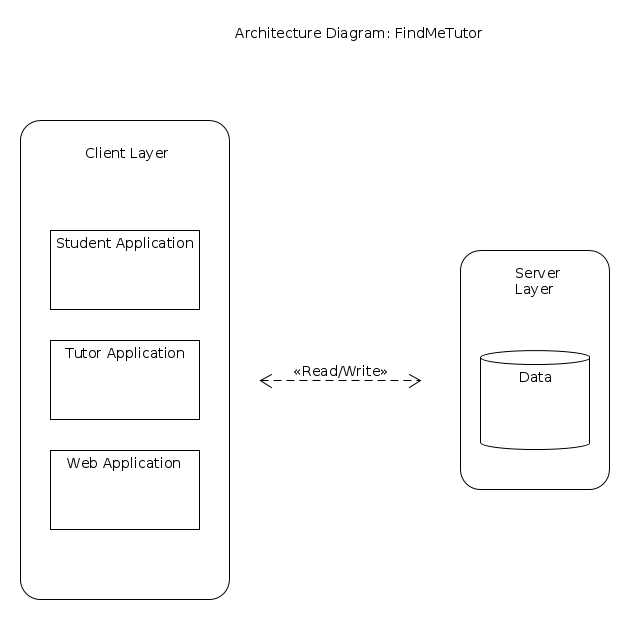
\includegraphics[width=140mm]{./architecture_diagram.png}
%\textbf{Put in diagram similar to above of sequence of how to request a tutor.}

\subsubsection{Class Diagram}
The class diagram below describes the structure of the FindMeTutor system. Showing the system classes, their attributes and relationships to one another.\\\\
The SQL database is stored on a linux based server hosted by Amazon Web Services apart from Amazon, FindMeTutor has ensured that we have a backup server hosted on the Microsoft Azure platform. 
\\\\
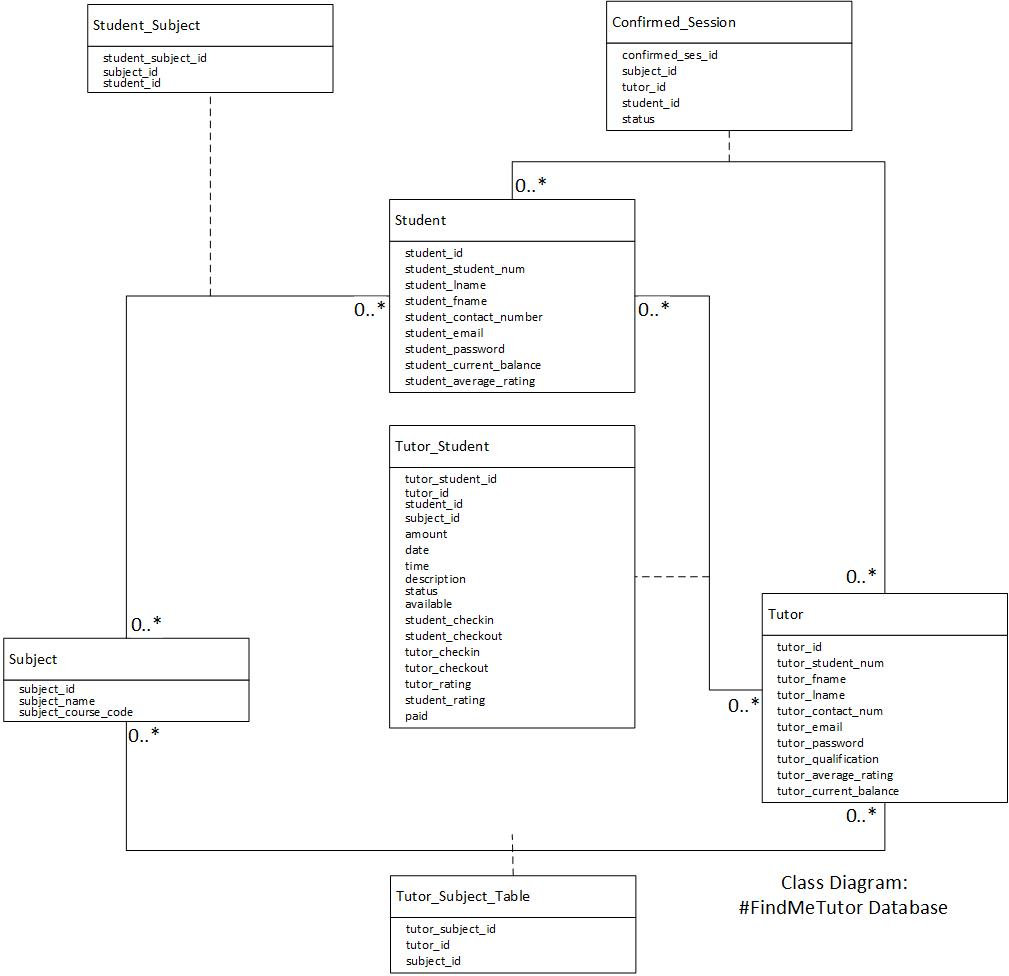
\includegraphics[width=140mm]{./class_diagram/class_diagram_findme_tutor.jpg}
\newpage

\subsubsection{Sequence Diagram}
Sequence Diagrams show the sequence of messages passed between objects of the FindMeTutor system over time.\\
\\\textbf{Create Student Sequence Diagram}:\\
The process of registering/creating a new student account on FindMeTutor using the student application.\\
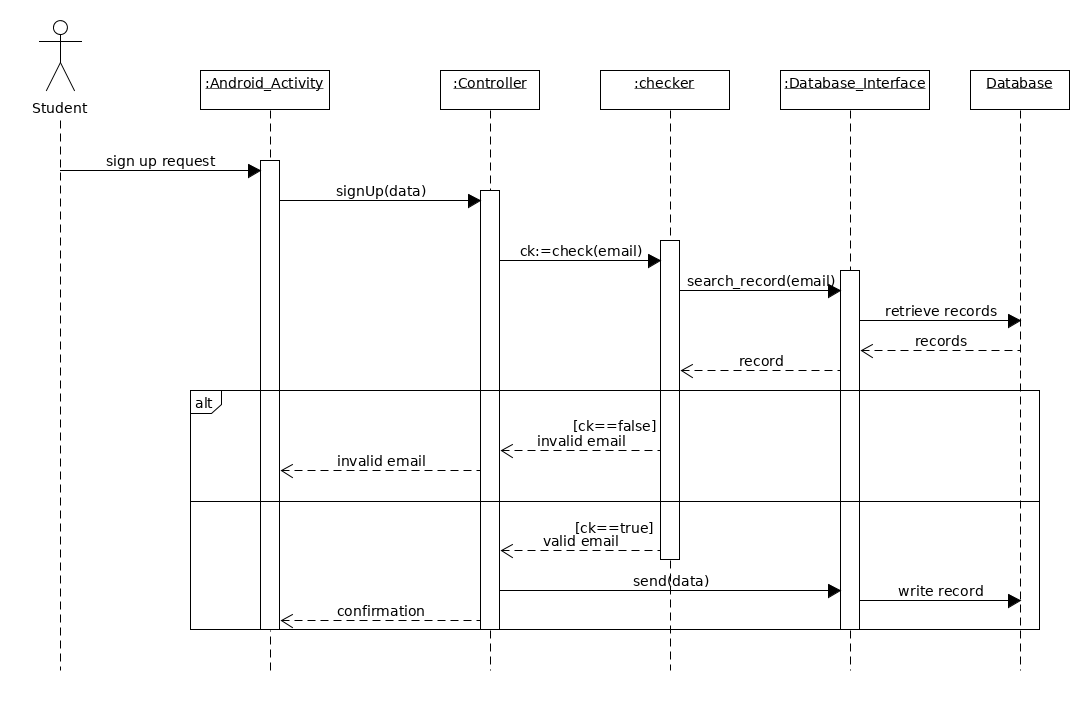
\includegraphics[width=140mm]{./sequence_diagram/create_student.png}
\newpage
\textbf{Request Tutor Sequence Diagram}:\\
The process of requesting a tutor on FindMeTutor using the student application.\\
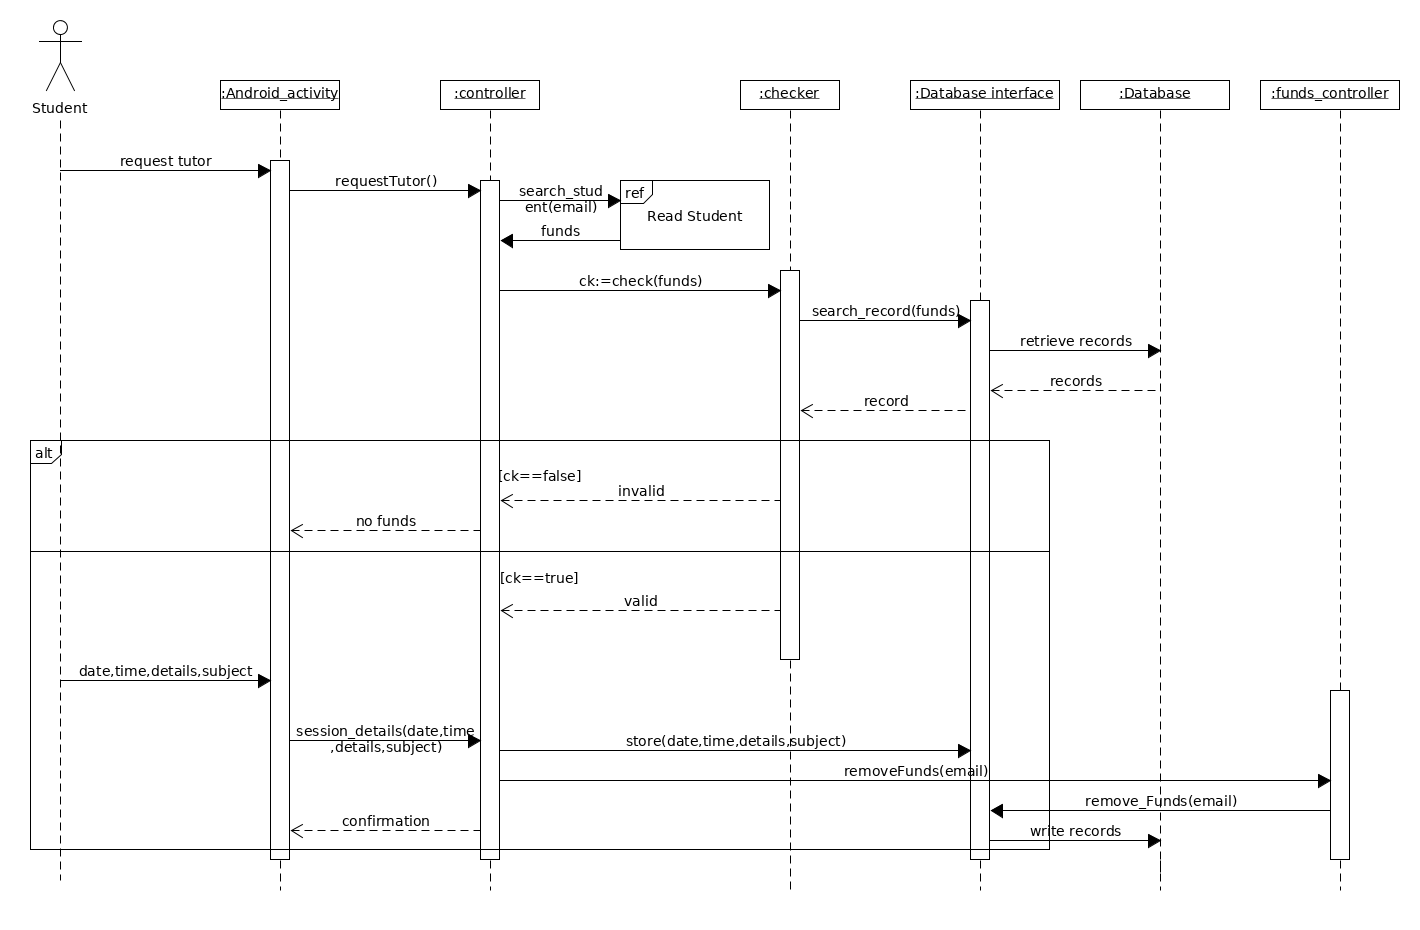
\includegraphics[width=140mm]{./sequence_diagram/request_tutor.png}
\newpage
\textbf{Add Subject Sequence Diagram}:\\
The process of adding a new subject on FindMeTutor using the student application.\\
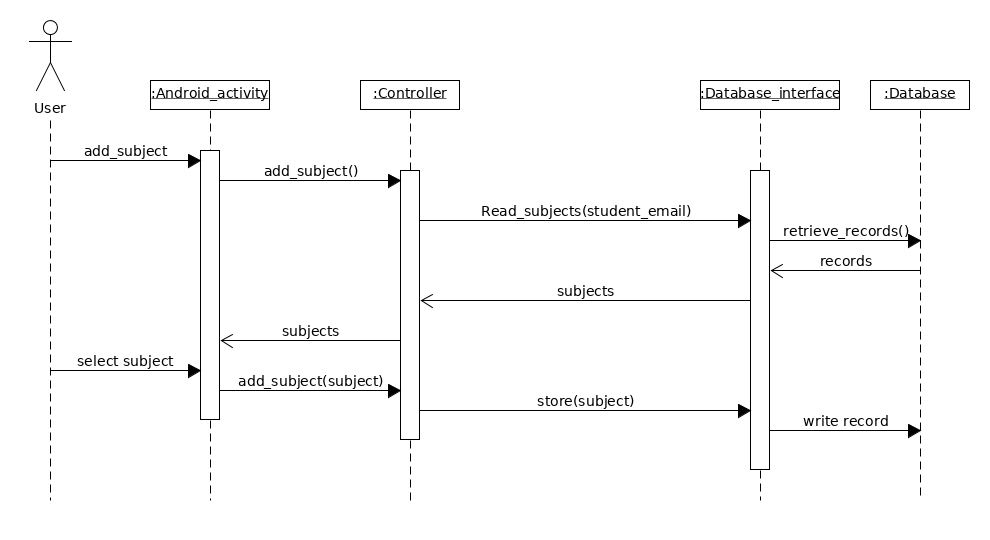
\includegraphics[width=140mm]{./sequence_diagram/add_subject.png}
\newpage
\textbf{Check In Sequence Diagram}:\\
The process of checking in a tutorial session.\\
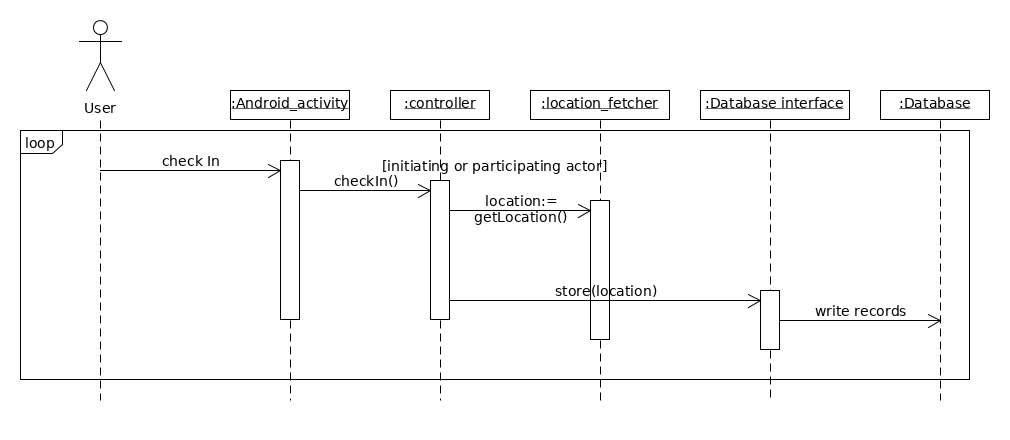
\includegraphics[width=140mm]{./sequence_diagram/check_in.png}
\newpage
\textbf{Check Out Sequence Diagram}:\\
The process of checking out of a tutorial session.\\
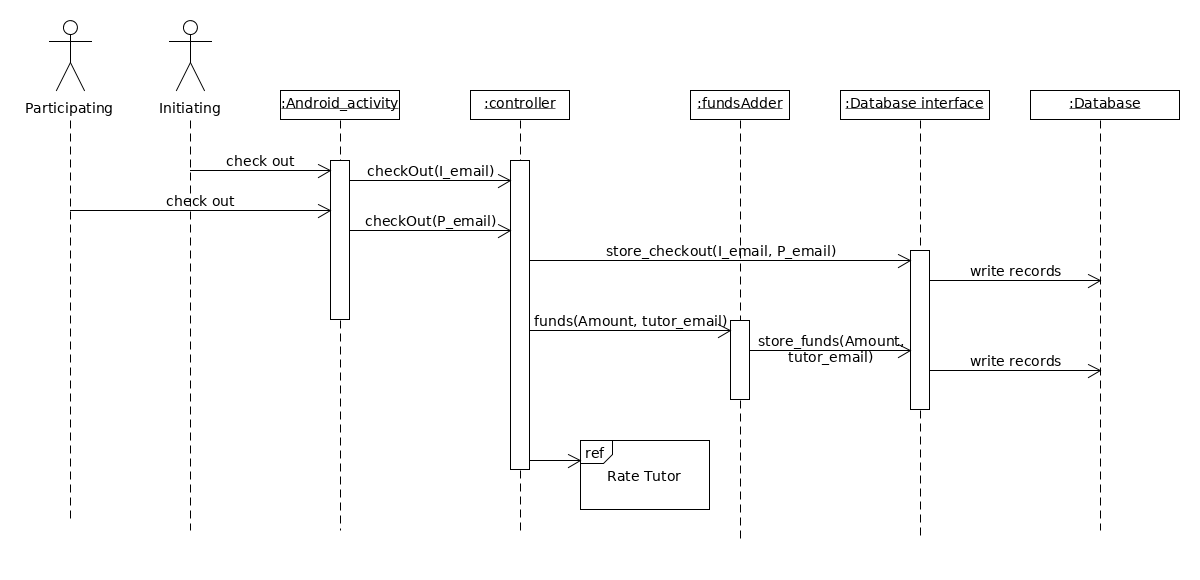
\includegraphics[width=140mm]{./sequence_diagram/check_out.png}
\newpage

\subsection{Development View}
The Development view outlines the components that are used to assemble the physical system.
The view addresses the concerns of stakeholders concerned with the development of system such as developers.\\
\\
Find Me Tutor is a mobile application built to run on Google's Android mobile operating system. Android is the currenty the biggest mobile operating system and we believe that it is the perfect platform for FindMeTutor.\\\\
There are two mobile applications that make up FindMeTutor. The first being the student application and the second being the tutor application. Students make use of the student application while Tutors make use of the tutor application.\\
\subsubsection{Package Diagram}

A package diagram depicts the dependencies the packages of the FindMeTutor system.
Below is package diagrams of the FindMeTutor system:\\
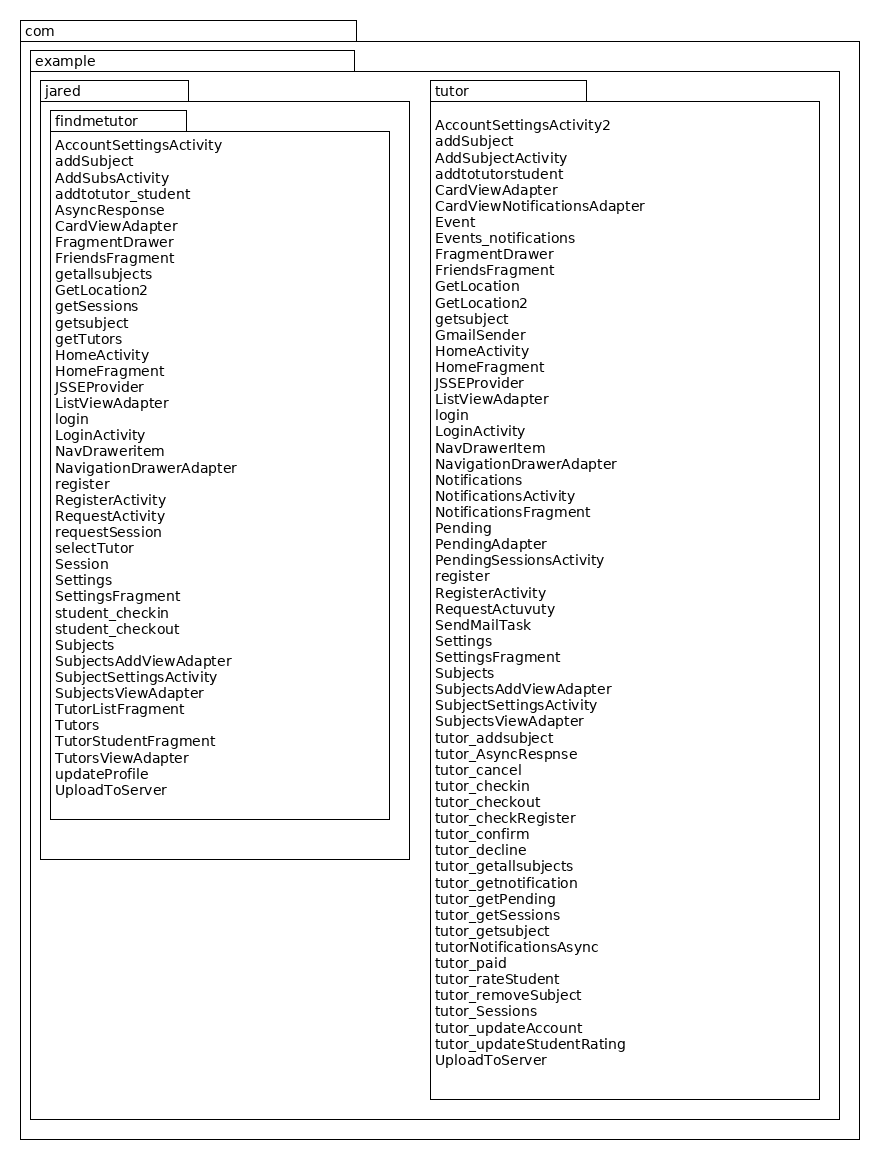
\includegraphics[width=140mm]{./package_diagram/package_diagram.png}


\subsubsection{Component Diagram}
A component diagram describes the components used to achieve the functionality of the FindMeTutor system.\\
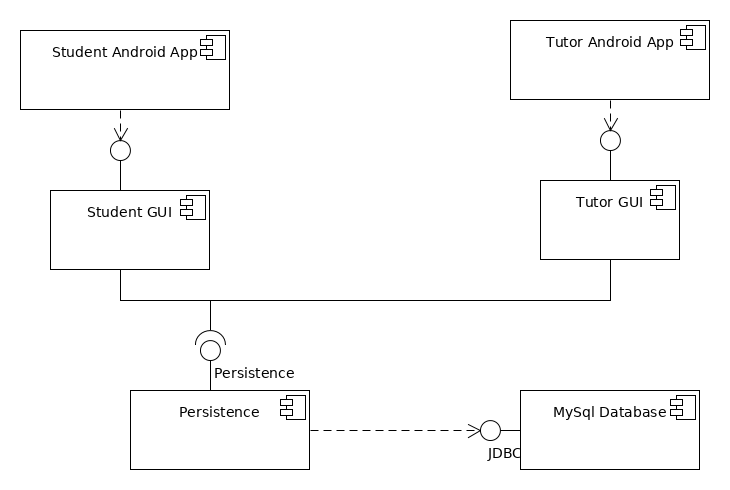
\includegraphics[width=140mm]{./component_diagram/component_diagram.png}

\newpage

\subsection{Process View}
The process view considers the non-functional aspects of the FindMeTutor system. It addresses the concerns of the stakeholders concerned with the design of the system.

\subsubsection{Activity Diagrams}
An activity diagram depicts the the flows of the system and business logic with actions.\\
\\\textbf{Request Tutor:}\\
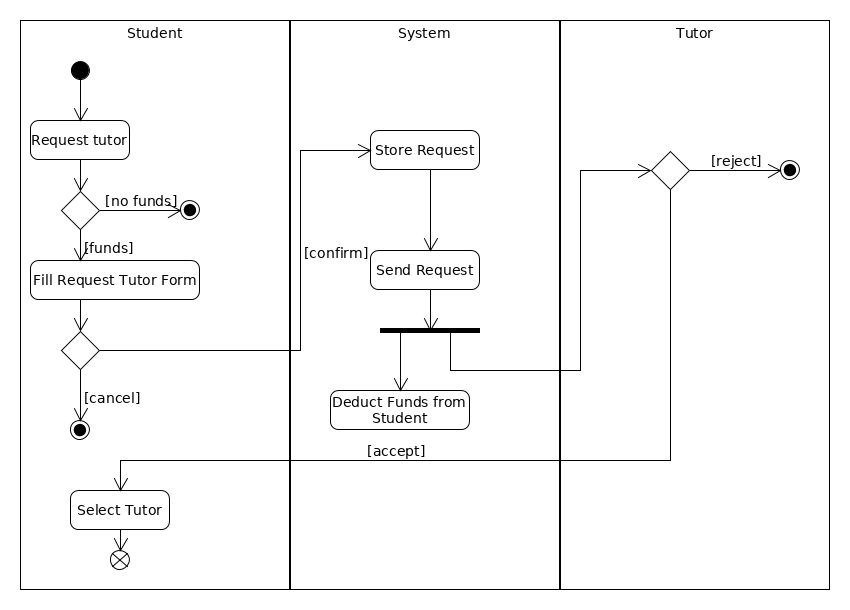
\includegraphics[width=140mm]{./activity_diagram/request_tutor.png}
\pagebreak
\\\\\textbf{Check In:}\\
The initiating actor is either a student or a tutor where a participating actor refers to a tutor or student.\\
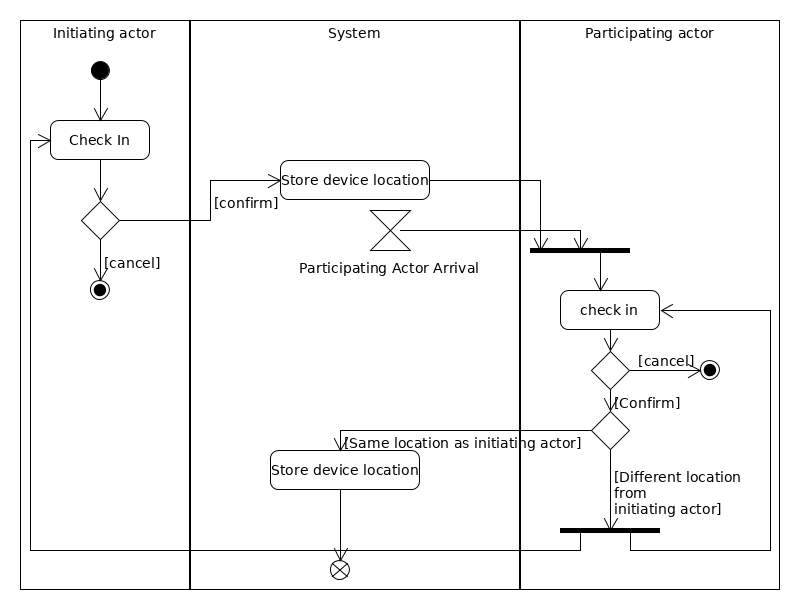
\includegraphics[width=140mm]{./activity_diagram/checked_in.png}
\pagebreak
\\\\\textbf{Rate Tutor:}\\
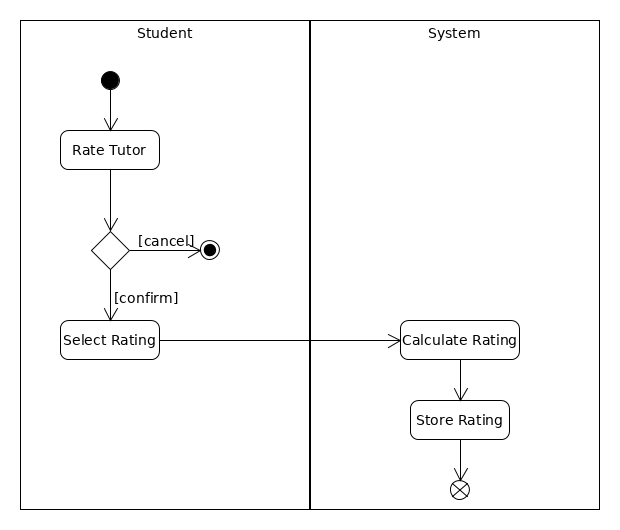
\includegraphics[width=140mm]{./activity_diagram/rate_tutor.png}
\\\\\textbf{Check Out:}\\
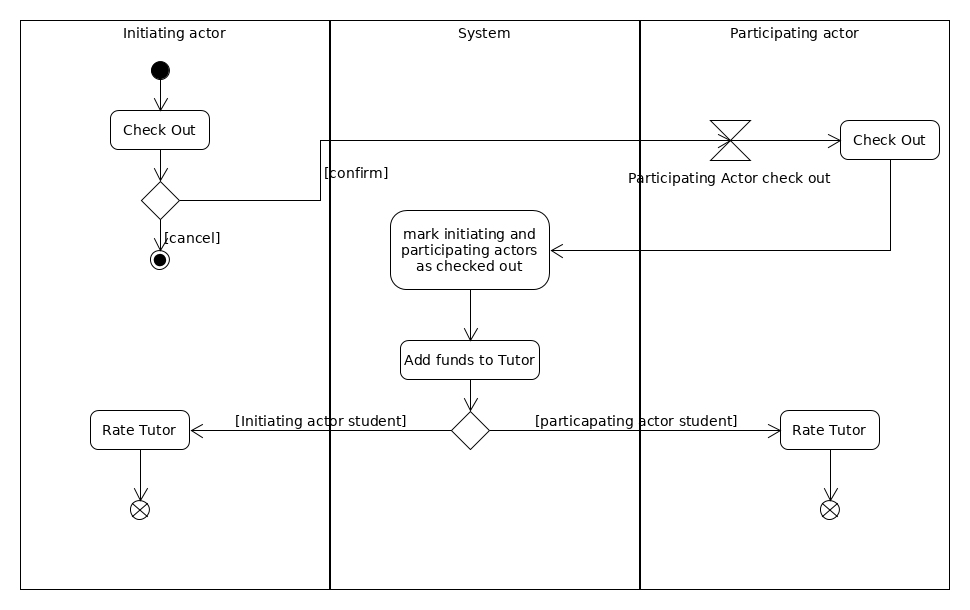
\includegraphics[width=140mm]{./activity_diagram/check_out.png}

\newpage
\subsubsection{Communication Diagrams}
The communication diagrams for Reqeust a Tutor, Create a Student Account and to add a Subject on the system are below:\\
\textbf{Request Tutor}\\
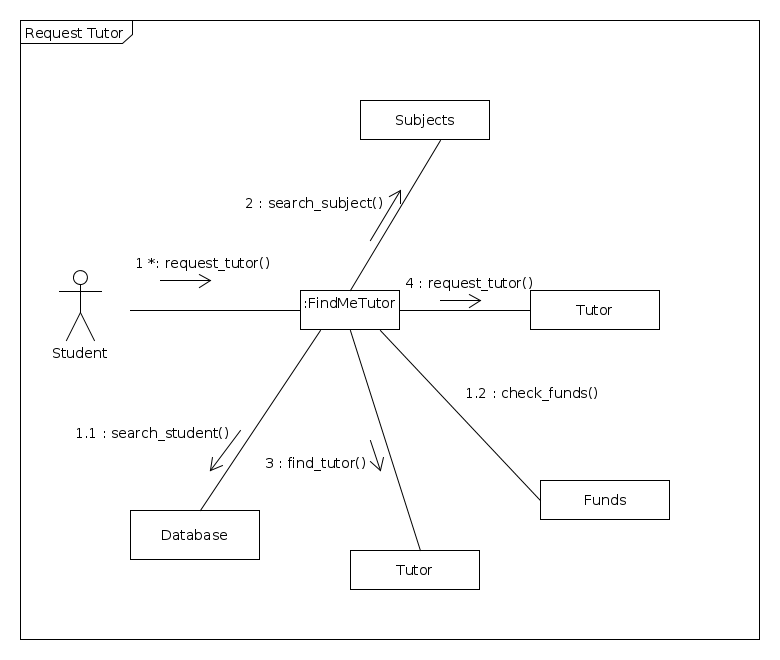
\includegraphics[width=140mm]{./communication_diagram/communication_diagram_rt.png}
%\newpage
\newpage
\textbf{Create Student}\\
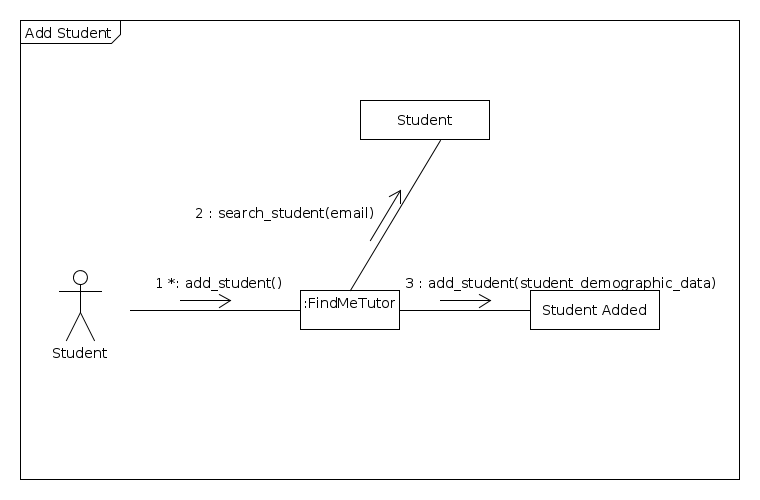
\includegraphics[width=140mm]{./communication_diagram/communication_diagram_cs.png}
\newpage
\textbf{Add Subject}\\
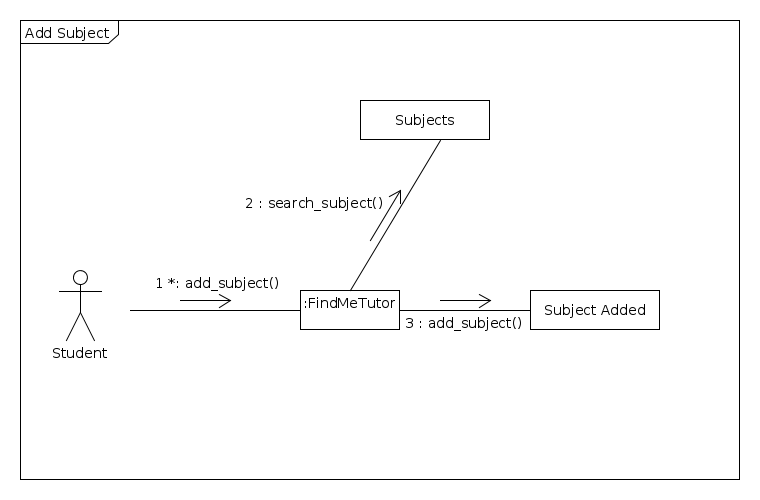
\includegraphics[width=140mm]{./communication_diagram/communication_diagram_as.png}
\newpage
\subsubsection{State Diagrams}
The most important state diagrams for the FindMeTutor system are listed below, they depict the states in which various attributes of the database change.\\

\textbf{State Diagram: "Status" in the Confrimed Session Table}\\\\
\text The state is changed when the tutor has accepted the tutoring session.
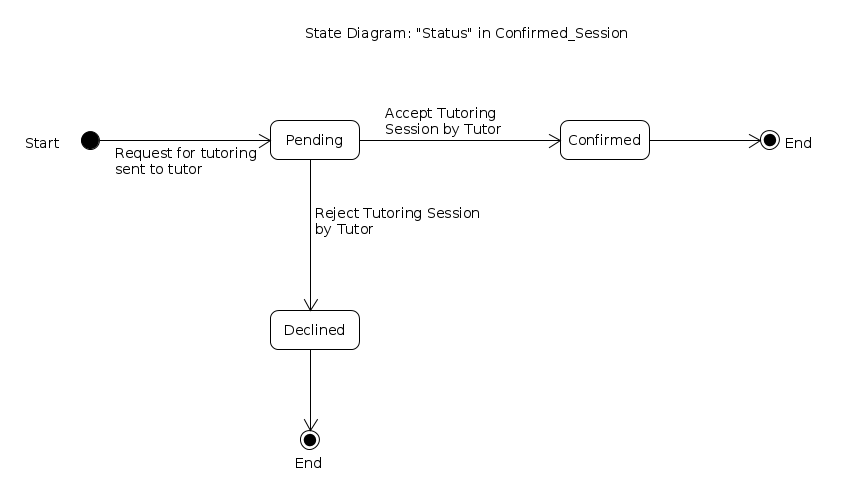
\includegraphics[width=140mm]{./state_diagram/statediagram_status.png}
\\
\textbf{State Diagram: "Paid" in the Tutor Student Table}\\\\
\text The state is changed when the student has paid for the tutoring session.
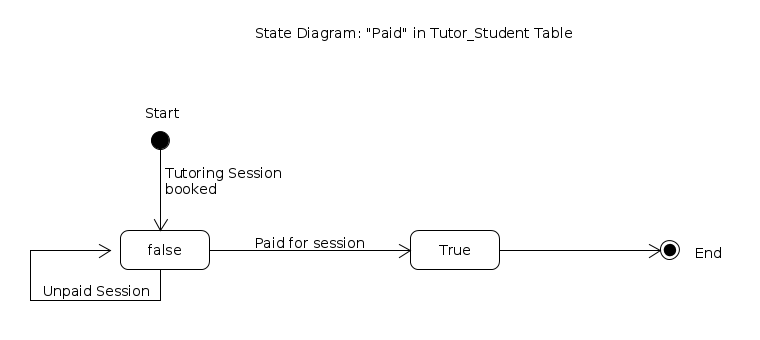
\includegraphics[width=140mm]{./state_diagram/statediagram_paid.png}


\newpage

\subsection{Physical View}
The physical view describes the physical locations of software, the scalability of the system, the deployment and installation.
\\\\
The server side of FindMetutor makes use of an SQL server, we have selected Amazon Web Services as our primary provider. We also have a backup server on the Microsoft Azure platform. \\\\
On the user side we have the mobile device running the latest version of Google's Android operating system. The application(s) are then installed on Android.\\
\subsubsection{Deployment Diagram}

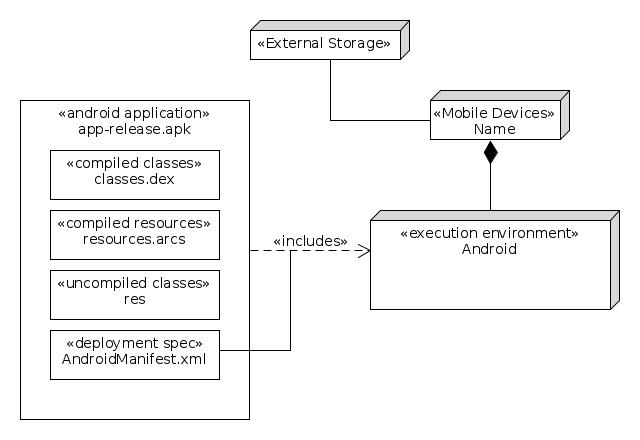
\includegraphics[width=140mm]{./Deployment.jpg}

\newpage

\subsection{Scenarios}
The Scenarios view address concerns of all stakeholders, this view helps show how the system is to be used.
\subsubsection{Use Case Diagram}
The use case diagram describes the behaviour of the system from the view of it's users.\\
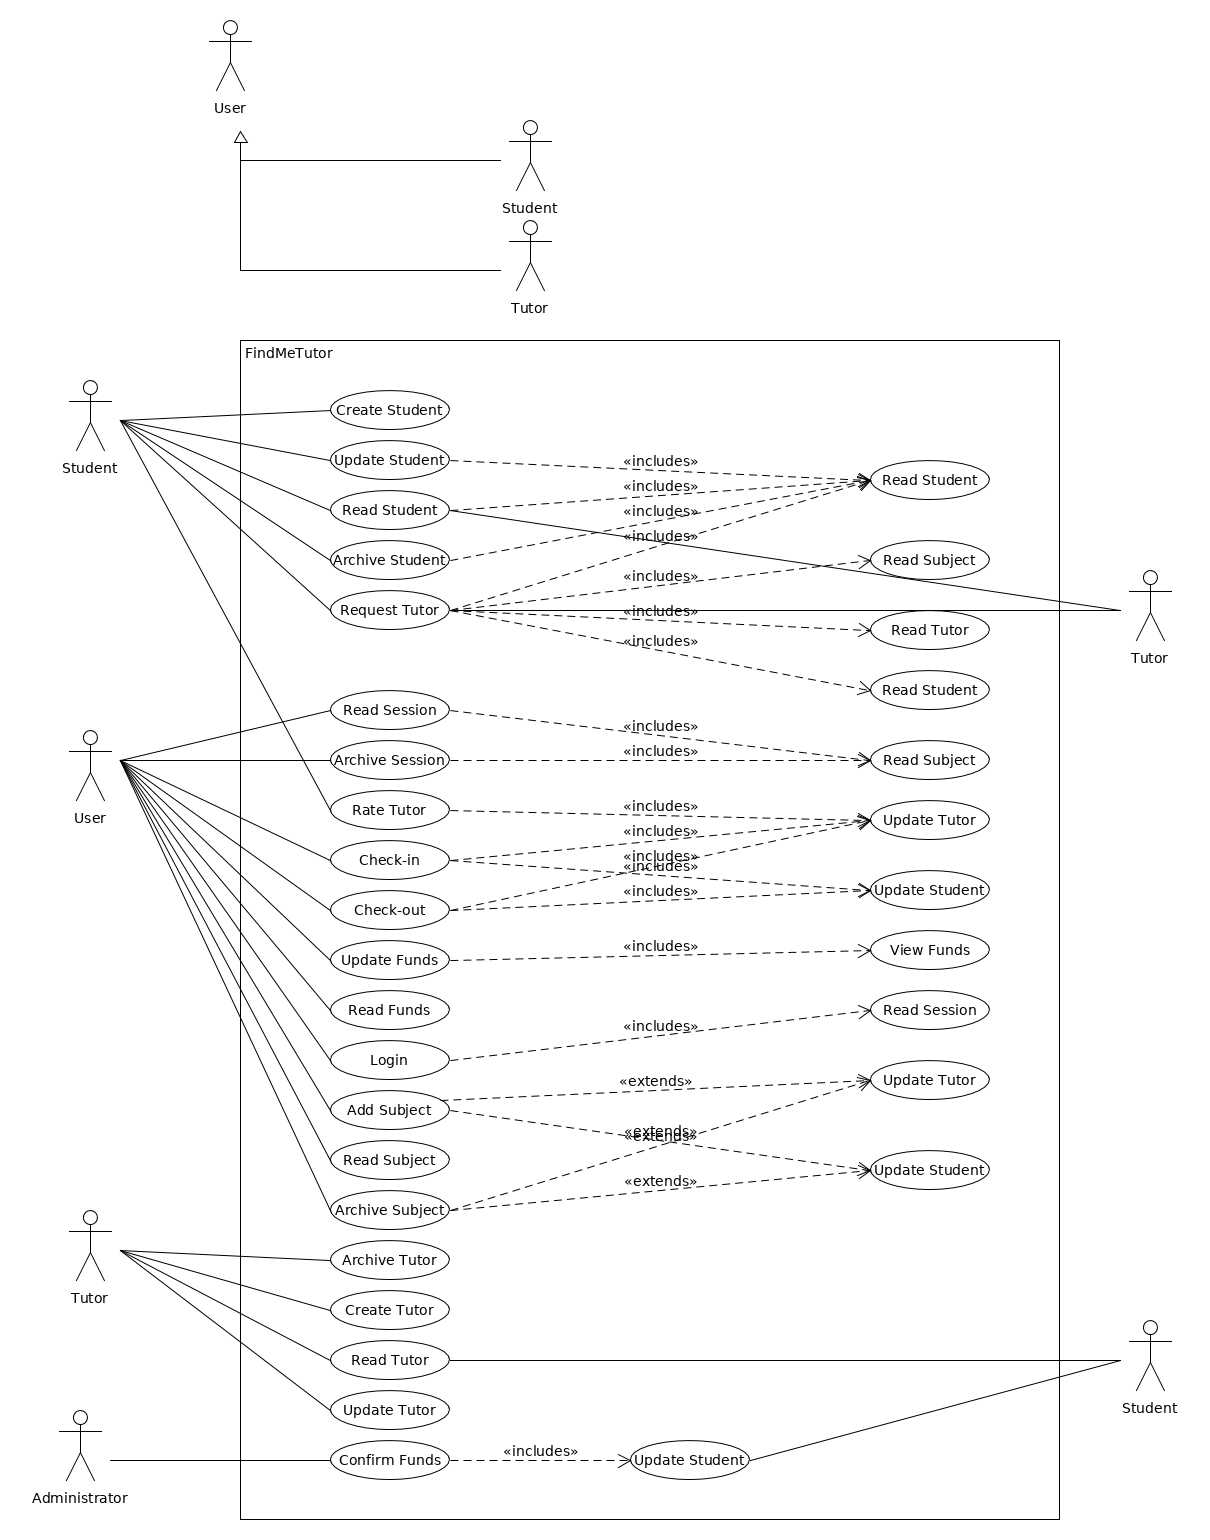
\includegraphics[width=170mm]{./Use_Case_Diagram.png}

\end{document}
